\documentclass[border=1pt]{standalone}
\usepackage{mathptmx}  % Times text and math
\usepackage{circuitikz}
\usetikzlibrary{arrows.meta}
\ctikzset{bipoles/length=0.75cm, transistors/scale=0.9,
  inductors/coils=4, current/distance=.5, bipoles/diode/height=.32,
  bipoles/diode/width=.26}
\begin{document}
\fontsize{8}{9.6}\selectfont
% foc_pmsm: control diagram, 1 layout unit = 1 cm (ieee-double)
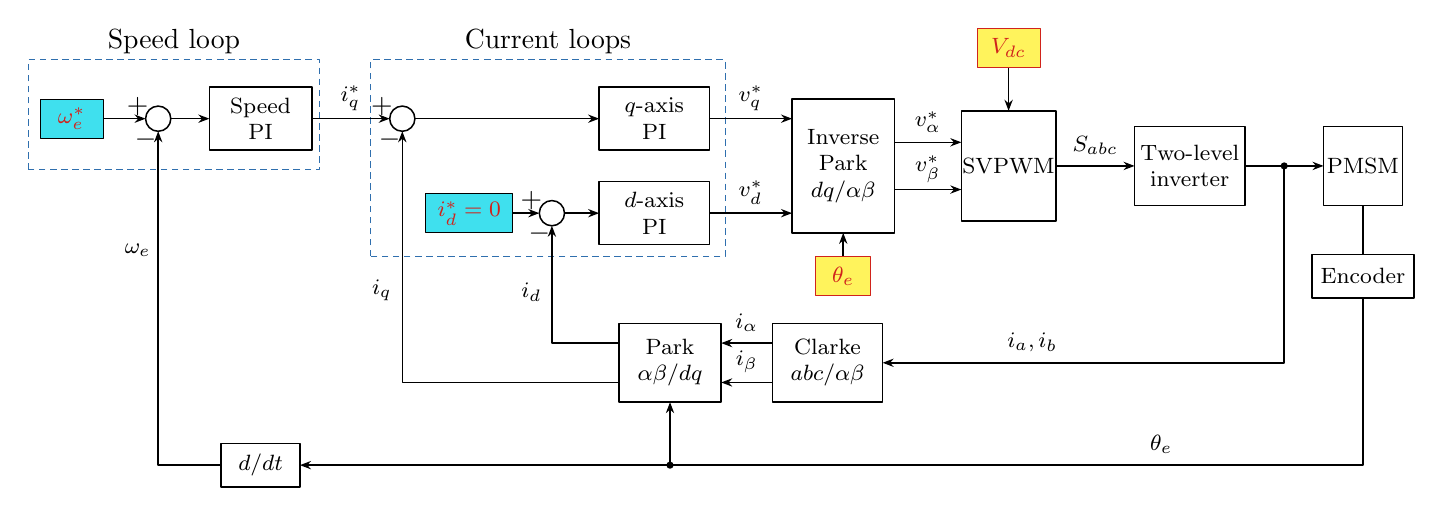
\begin{tikzpicture}[x=1cm, y=1cm, line width=0.55pt, line join=round]
% ---- regions (background) ----
\draw[draw={rgb,255:red,47;green,111;blue,174}, line width=0.44pt, dash pattern=on 2.4pt off 1.6pt] (0.05,0.55) rectangle (3.75,1.95);
\node[inner sep=0pt] at (1.9,2.18) {Speed loop};
\draw[draw={rgb,255:red,47;green,111;blue,174}, line width=0.44pt, dash pattern=on 2.4pt off 1.6pt] (4.4,-0.55) rectangle (8.9,1.95);
\node[inner sep=0pt] at (6.65,2.18) {Current loops};
% ---- links ----
\draw[-{Stealth[length=0.14cm]}] (1,1.2) -- (1.54,1.2);
\draw[-{Stealth[length=0.14cm]}] (1.86,1.2) -- (2.35,1.2);
\draw[-{Stealth[length=0.14cm]}] (3.65,1.2) -- (4.64,1.2);
\draw[-{Stealth[length=0.14cm]}] (4.96,1.2) -- (7.3,1.2);
\draw[-{Stealth[length=0.14cm]}] (6.2,0) -- (6.54,0);
\draw[-{Stealth[length=0.14cm]}] (6.86,0) -- (7.3,0);
\draw[-{Stealth[length=0.14cm]}] (8.7,1.2) -- (9.75,1.2);
\draw[-{Stealth[length=0.14cm]}] (8.7,0) -- (9.75,0);
\draw[-{Stealth[length=0.14cm]}] (10.4,-0.55) -- (10.4,-0.25);
\draw[-{Stealth[length=0.14cm]}] (11.05,0.9) -- (11.9,0.9);
\draw[-{Stealth[length=0.14cm]}] (11.05,0.3) -- (11.9,0.3);
\draw[-{Stealth[length=0.14cm]}] (12.5,1.85) -- (12.5,1.3);
\draw[-{Stealth[length=0.14cm]}] (13.1,0.6) -- (14.1,0.6);
\draw[-{Stealth[length=0.14cm]}] (15.5,0.6) -- (16.5,0.6);
\draw[-{Stealth[length=0.14cm]}] (16,0.6) -- (16,-1.9) -- (10.9,-1.9);
\draw[-{Stealth[length=0.14cm]}] (9.5,-1.65) -- (8.85,-1.65);
\draw[-{Stealth[length=0.14cm]}] (9.5,-2.15) -- (8.85,-2.15);
\draw (17,0.1) -- (17,-0.525);
\draw[-{Stealth[length=0.14cm]}] (17,-1.075) -- (17,-3.2) -- (3.5,-3.2);
\draw[-{Stealth[length=0.14cm]}] (8.2,-3.2) -- (8.2,-2.4);
\draw[-{Stealth[length=0.14cm]}] (7.55,-1.65) -- (6.7,-1.65) -- (6.7,-0.16);
\draw[-{Stealth[length=0.14cm]}] (7.55,-2.15) -- (4.8,-2.15) -- (4.8,1.04);
\draw[-{Stealth[length=0.14cm]}] (2.5,-3.2) -- (1.7,-3.2) -- (1.7,1.04);
% ---- branch dots ----
\fill (16,0.6) circle (1.3pt);
\fill (8.2,-3.2) circle (1.3pt);
% ---- wref (tag) ----
\filldraw[fill={rgb,255:red,63;green,224;blue,238}, draw={rgb,255:red,0;green,0;blue,0}, line width=0.33pt] (0.2,0.95) rectangle (1,1.45);
% ---- sw (sum) ----
\draw[fill=white] (1.7,1.2) circle (0.16cm);
% ---- piw (block) ----
\draw[fill=white] (2.35,0.8) rectangle (3.65,1.6);
% ---- sq (sum) ----
\draw[fill=white] (4.8,1.2) circle (0.16cm);
% ---- idref (tag) ----
\filldraw[fill={rgb,255:red,63;green,224;blue,238}, draw={rgb,255:red,0;green,0;blue,0}, line width=0.33pt] (5.1,-0.25) rectangle (6.2,0.25);
% ---- sd (sum) ----
\draw[fill=white] (6.7,0) circle (0.16cm);
% ---- piq (block) ----
\draw[fill=white] (7.3,0.8) rectangle (8.7,1.6);
% ---- pid (block) ----
\draw[fill=white] (7.3,-0.4) rectangle (8.7,0.4);
% ---- ipark (block) ----
\draw[fill=white] (9.75,-0.25) rectangle (11.05,1.45);
% ---- thi (tag) ----
\filldraw[fill={rgb,255:red,255;green,243;blue,92}, draw={rgb,255:red,208;green,35;blue,28}, line width=0.33pt] (10.05,-1.05) rectangle (10.75,-0.55);
% ---- vdc (tag) ----
\filldraw[fill={rgb,255:red,255;green,243;blue,92}, draw={rgb,255:red,208;green,35;blue,28}, line width=0.33pt] (12.1,1.85) rectangle (12.9,2.35);
% ---- svpwm (block) ----
\draw[fill=white] (11.9,-0.1) rectangle (13.1,1.3);
% ---- inv (block) ----
\draw[fill=white] (14.1,0.1) rectangle (15.5,1.1);
% ---- pmsm (block) ----
\draw[fill=white] (16.5,0.1) rectangle (17.5,1.1);
% ---- enc (block) ----
\draw[fill=white] (16.35,-1.075) rectangle (17.65,-0.525);
% ---- park (block) ----
\draw[fill=white] (7.55,-2.4) rectangle (8.85,-1.4);
% ---- clarke (block) ----
\draw[fill=white] (9.5,-2.4) rectangle (10.9,-1.4);
% ---- ddt (block) ----
\draw[fill=white] (2.5,-3.475) rectangle (3.5,-2.925);
% ---- signs ----
\node[inner sep=0pt] at (1.44,1.36) {$+$};
\node[inner sep=0pt] at (1.54,0.94) {$-$};
\node[inner sep=0pt] at (4.54,1.36) {$+$};
\node[inner sep=0pt] at (4.64,0.94) {$-$};
\node[inner sep=0pt] at (6.44,0.16) {$+$};
\node[inner sep=0pt] at (6.54,-0.26) {$-$};
% ---- text ----
\node[inner sep=0pt, align=center, font=\fontsize{8}{9.6}\selectfont, text={rgb,255:red,208;green,35;blue,28}] at (0.6,1.2) {$\omega_{e}^{*}$};
\node[inner sep=0pt, align=center, font=\fontsize{8}{9.6}\selectfont] at (3,1.2) {Speed\\PI};
\node[inner sep=0pt, align=center, font=\fontsize{8}{9.6}\selectfont, text={rgb,255:red,208;green,35;blue,28}] at (5.65,0) {$i_{d}^{*}=0$};
\node[inner sep=0pt, align=center, font=\fontsize{8}{9.6}\selectfont] at (8,1.2) {$q$-axis\\PI};
\node[inner sep=0pt, align=center, font=\fontsize{8}{9.6}\selectfont] at (8,0) {$d$-axis\\PI};
\node[inner sep=0pt, align=center, font=\fontsize{8}{9.6}\selectfont] at (10.4,0.6) {Inverse\\Park\\$dq/\alpha\beta$};
\node[inner sep=0pt, align=center, font=\fontsize{8}{9.6}\selectfont, text={rgb,255:red,208;green,35;blue,28}] at (10.4,-0.8) {$\theta_{e}$};
\node[inner sep=0pt, align=center, font=\fontsize{8}{9.6}\selectfont, text={rgb,255:red,208;green,35;blue,28}] at (12.5,2.1) {$V_{dc}$};
\node[inner sep=0pt, align=center, font=\fontsize{8}{9.6}\selectfont] at (12.5,0.6) {SVPWM};
\node[inner sep=0pt, align=center, font=\fontsize{8}{9.6}\selectfont] at (14.8,0.6) {Two-level\\inverter};
\node[inner sep=0pt, align=center, font=\fontsize{8}{9.6}\selectfont] at (17,0.6) {PMSM};
\node[inner sep=0pt, align=center, font=\fontsize{8}{9.6}\selectfont] at (17,-0.8) {Encoder};
\node[inner sep=0pt, align=center, font=\fontsize{8}{9.6}\selectfont] at (8.2,-1.9) {Park\\$\alpha\beta/dq$};
\node[inner sep=0pt, align=center, font=\fontsize{8}{9.6}\selectfont] at (10.2,-1.9) {Clarke\\$abc/\alpha\beta$};
\node[inner sep=0pt, align=center, font=\fontsize{8}{9.6}\selectfont] at (3,-3.2) {$d/dt$};
\node[inner sep=0pt, align=center, font=\fontsize{8}{9.6}\selectfont] at (4.145,1.46) {$i_{q}^{*}$};
\node[inner sep=0pt, align=center, font=\fontsize{8}{9.6}\selectfont] at (9.225,1.46) {$v_{q}^{*}$};
\node[inner sep=0pt, align=center, font=\fontsize{8}{9.6}\selectfont] at (9.225,0.26) {$v_{d}^{*}$};
\node[inner sep=0pt, align=center, font=\fontsize{8}{9.6}\selectfont] at (11.475,1.16) {$v_{\alpha}^{*}$};
\node[inner sep=0pt, align=center, font=\fontsize{8}{9.6}\selectfont] at (11.475,0.56) {$v_{\beta}^{*}$};
\node[inner sep=0pt, align=center, font=\fontsize{8}{9.6}\selectfont] at (13.6,0.86) {$S_{abc}$};
\node[inner sep=0pt, align=center, font=\fontsize{8}{9.6}\selectfont] at (12.8,-1.64) {$i_{a}, i_{b}$};
\node[inner sep=0pt, align=center, font=\fontsize{8}{9.6}\selectfont] at (9.175,-1.39) {$i_{\alpha}$};
\node[inner sep=0pt, align=center, font=\fontsize{8}{9.6}\selectfont] at (9.175,-1.89) {$i_{\beta}$};
\node[inner sep=0pt, align=center, font=\fontsize{8}{9.6}\selectfont] at (14.4375,-2.94) {$\theta_{e}$};
\node[inner sep=0pt, align=center, font=\fontsize{8}{9.6}\selectfont] at (6.44,-1.0024) {$i_{d}$};
\node[inner sep=0pt, align=center, font=\fontsize{8}{9.6}\selectfont] at (4.54,-0.9796) {$i_{q}$};
\node[inner sep=0pt, align=center, font=\fontsize{8}{9.6}\selectfont] at (1.44,-0.472) {$\omega_{e}$};
\end{tikzpicture}
\end{document}
